% !TeX spellcheck = nl_NL
\documentclass{article}

\begin{document}
	\subsection{Dispatcher}
	\subsubsection{Het nut van een dispatcher}
	De dispatcher is AEM's eigen caching laag en dient als publieke gateway voor de gebruikers. Doordat de publieke requests via de dispatcher gaan voorziet deze een extra beveiligingslaag. Dit door het feit dat we AEM kunnen afschermen voor requests van buiten ons netwerk. Om een dispatcher op te zetten installeren we de module op een web server en configureren deze. Deze configuratie bevat, onder anderen, waar onze AEM draait, welke soort bestanden er gecached moeten worden en hoe de cache van deze bestanden vervalt.
	\par	
	 Wanneer een dispatcher een request binnen krijgt wordt deze eerst geanalyseerd of deze in aanmerking komt voor onze cache. Buiten onze configuratie zijn er ook enkele standaard regels waarna gekeken wordt om dit te bepalen. Enkel de HTTP methode GET komt in aanmerking voor de cache, indien het request een andere methode bevat kan deze niet gecached worden. Ook wanneer er een request parameter wordt meegegeven kan de request niet gecached worden aangezien zo'n request een variabel antwoord heeft.
	\par
	Er zijn vier manieren waarop een cache kan vervallen, de eerste zijnde een levensduur aan de caches toekennen. Wanneer een cache deze levensduur overschrijdt vervalt deze, bij een volgend request wordt er een nieuwe call naar de publisher gedaan. Deze nieuwe versie vervangt vervolgens de oude cache en wordt naar de gebruiker doorgestuurd.
	\par
	Een andere mogelijkheid is om de cache van een pagina te verwijderen wanneer een nieuwe versie beschikbaar wordt. Hiervoor moet de author een flush request doen naar de dispatcher toe op het moment dat een pagina wordt gepublished. Dit request verwijdert de cache, de volgende keer dat de pagina wordt opgevraagd is de dispatcher verplicht om deze opnieuw op te halen.
	\par
	 Een andere manier om bij het publiceren een cache te invalideren is met het gebruik van stat bestanden. Een stat bestand is een record dat (onder andere) de laatste datum van modificatie onthoudt. Wanneer een pagina wordt gepubliceerd, plaats de author een stat bestand voor deze pagina op de dispatcher. Het tijdstip van modificatie van het stat bestand zal telkens vergeleken worden met die van de gecachte pagina. Indien die van de pagina ouder is, weet de dispatcher dat er een nieuwe versie beschikbaar is. Vervolgens verwijdert de dispatcher de cache en haalt de nieuwe versie op.
	 \par
	 Een laatste techniek is het expliciet verwijderen van de bestanden op de dispatcher. Deze zal niet meer in staat zijn de pagina terug te vinden en wordt verplicht om deze opnieuw op te halen. Dit kan manueel gebeuren door in te loggen op de machine of via een script dat periodiek wordt uitgevoerd.
	\subsubsection{Een dispatcher opzetten}
	Een dispatcher is niet meer dan een module die draait op een webserver. Om deze module te gebruiken hebben we dus, buiten Java, nog een webserver nodig. We installeren de Apache webserver op de machine waar we onze dispatcher willen draaien. Dit doen we door twee commando's uit te voeren.
	\begin{lstlisting}
		 $ sudo yum update
		 $ sudo yum install httpd
	\end{lstlisting}
	We voorzien een folder dispatcher en downloaden hierin de tar van de gewenste versie.
	\begin{lstlisting}
		 $ wget https://www.adobeaemcloud.com/content/companies/public/adobe/dispatcher/		 dispatcher/_jcr_content/top/download_1/file.res/dispatcher-apache2.4-aix-powerpc-4.2.2.tar.gz
	\end{lstlisting}
	Vervolgens pakken we deze uit en verplaatsen het uitgepakte ".so" bestand naar de modules folder van Apache.
	\begin{lstlisting}
		 $ tar -xvf dispatcher-apache2.4-aix-powerpc-4.2.2.tar.gz
		 $ sudo mv dispatcher-apache2.4-4.2.2.so /etc/httpd/modules/mod_dispatcher.so
	\end{lstlisting}
	We verplaatsen het dispatcher.any bestand naar de conf-folder van Apache.
	\begin{lstlisting}
		 $ cp dispatcher.any /etc/httpd/conf/dispatcher.any
	\end{lstlisting}
	We voorzien het /etc/httpd/conf/httpd.conf bestand met volgende lijnen, hierdoor weet Apache waar de module zich bevindt, waar de logs moeten worden weggeschreven en het pad naar het configuratiebestand voor deze module.
	\begin{figure}[h!]
  		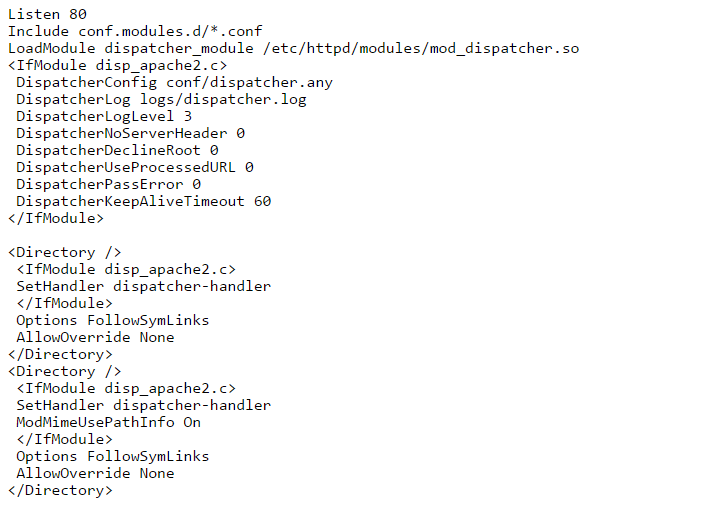
\includegraphics[width=\linewidth]{images/httpd-conf.PNG}
  		\caption{httpd.conf}
  		\label{fig:httpd.conf}
	\end{figure}
	\par
	\begin{figure}[h!]
  		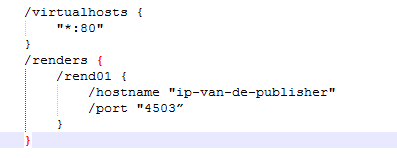
\includegraphics[width=\linewidth]{images/dispatcher-any.PNG}
  		\caption{dispatcher.any}
  		\label{fig:dispatcher-any}
	\end{figure}
	De laatste stap is de dispatcher laten weten waar onze publisher zich bevindt, dit doen we door de dispatcher.any file te voorzien van de configuratie uit Figuur \ref{fig:dispatcher-any}. De "virtualhosts" propertie kan gebruikt worden voor het beheren van meerdere sites door \'e\'en dispatcher. We kunnen meerdere hosts defini\"eren en elk voorzien van, onder andere, aparte renders (dus persoonlijke dispatchers) alsook ander gedrag voor de caching instellen. De "renders" propertie is de verzameling van publishers die we ter beschikking stellen, in dit geval hebben we er eentje: rend01. Bij commerci\"ele sites gaan dit er meer zijn, in dat geval zal de dispatcher zijn request verdelen over de beschikbare renders.
	
\end{document}